\documentclass[RNAAS]{aastex631}

% Numbers are \input from the pipeline-generated macros -- none typed by hand.
% Auto-generated by jansky_research.atlas3i.survey_macros — do not edit by hand.
\newcommand{\aiTotNodes}{60}
\newcommand{\aiTotScans}{360}
\newcommand{\aiTotBands}{4}
\newcommand{\aiTotRawHits}{1\,938\,860}
\newcommand{\aiTotSurvivors}{294}
\newcommand{\aiTotConfirmed}{0}
\newcommand{\aiSatCoherent}{9}
\newcommand{\aiEirpMw}{99.2}
\newcommand{\aiDistanceAu}{1.798}
\newcommand{\aiLNodes}{6}
\newcommand{\aiLBandLo}{939}
\newcommand{\aiLBandHi}{2064}
\newcommand{\aiLRawHits}{1\,124\,011}
\newcommand{\aiLSurvivors}{261}
\newcommand{\aiLConfirmed}{0}
\newcommand{\aiSNodes}{6}
\newcommand{\aiSBandLo}{1652}
\newcommand{\aiSBandHi}{2776}
\newcommand{\aiSRawHits}{354\,423}
\newcommand{\aiSSurvivors}{29}
\newcommand{\aiSConfirmed}{0}
\newcommand{\aiCNodes}{23}
\newcommand{\aiCBandLo}{3939}
\newcommand{\aiCBandHi}{8252}
\newcommand{\aiCRawHits}{15\,735}
\newcommand{\aiCSurvivors}{0}
\newcommand{\aiCConfirmed}{0}
\newcommand{\aiXNodes}{25}
\newcommand{\aiXBandLo}{7689}
\newcommand{\aiXBandHi}{12376}
\newcommand{\aiXRawHits}{444\,691}
\newcommand{\aiXSurvivors}{4}
\newcommand{\aiXConfirmed}{0}


\newcommand{\code}[1]{\texttt{#1}}

\begin{document}

\title{An Independent Reproduction of the Breakthrough Listen 3I/ATLAS L-band
Nondetection from the Public Green Bank Telescope Data}

\author[0009-0008-3289-4447]{Joseph Barbere}
\affiliation{Independent researcher}

\begin{abstract}
Breakthrough Listen's technosignature search of the interstellar object 3I/ATLAS with
the Green Bank Telescope reported a nondetection down to $\sim$100~mW equivalent
isotropic radiated power \citep{jacobsonbell2025}, and released the data publicly. I
reprocess the L-band cadence with an independent, open pipeline --- a physical-units
de-Doppler search, the ABACAD on/off filter, and a per-candidate drift-coherence vet
--- and reproduce the null: \aiRawHits\ raw hits reduce to \aiSurvivors\ two-position
survivors and \aiConfirmed\ confirmed candidates, with a matching
\aiEirpMw~mW limit. The survivors that evade each filter stage are themselves
instructive: sub-threshold terrestrial carriers, and satellite downlinks that defeat
any two-position sky filter by design.
\end{abstract}

\section{Result}

On 2025 December 18 Breakthrough Listen observed 3I/ATLAS with the GBT in four bands
(1--12~GHz) using 6$\times$5-min ABACAD on/off cadences, searched the fine-resolution
($\sim$2.8~Hz) data with \code{turboSETI} over $\pm4$~Hz\,s$^{-1}$, and found no
technosignature candidates \citep{jacobsonbell2025}. Companion searches with the ATA
\citep{ata3i} and FAST \citep{fast3i} also report nulls. All GBT data are public
(\url{https://bldata.berkeley.edu/ATLAS}), yet --- as for most technosignature nulls
--- no independent reanalysis of the released files existed.

\code{atlas3i} \citep{janskyresearch} is such a reanalysis for the L-band cadence
(\aiNodes\ compute-node sub-bands spanning \aiBandLo--\aiBandHi~MHz; the paper analyses
1.1--1.9~GHz within this recorded span): a brute-force shift-and-sum de-Doppler search
in physical units over $\pm4$~Hz\,s$^{-1}$, with per-channel bandpass normalization and
DC-spike excision, thresholded at $16\sigma$ against per-drift-rate robust (MAD) noise;
an on/off filter requiring a hit to appear, extrapolated along its own drift rate, in
every on-target scan and no off-target scan; and a postage-stamp vet that re-reads all
six scans around each survivor and demands the same coherence directly of the data.
Every stage is validated offline on a synthetic cadence with an injected drifting tone,
an always-on interferer, and a DC spike.

The result reproduces the paper's null (Figure~\ref{fig:sweep}): \aiRawHits\ raw hits
$\to$ \aiSurvivors\ two-position survivors $\to$ \aiConfirmed\ confirmed. The
$16\sigma$ narrowband limit, $\mathrm{EIRP} = 4\pi d^{2}\,S_\mathrm{min}\,\delta\nu$
with the paper's own parameters (SEFD $\approx$ 10~Jy, 300~s scans,
$d=\aiDistanceAu$~au from JPL Horizons at the cadence epoch), is
$\mathrm{EIRP} \le \aiEirpMw$~mW --- algebraically identical to the paper's formulation
\citep{gajjar2021} for unit dedrifting efficiency, hence the matching $\sim$100~mW.

\section{What Evades a Two-Position Filter}

The vetted survivors are a taxonomy of filter evasion. Terrestrial carriers at
1302--1308~MHz (aeronautical radionavigation) passed the on/off filter by sitting below
the search threshold in the off scans; the stamp vet sees them there directly.
High-drift survivors cluster in GNSS allocations (GPS L5/Galileo E5) and fail
drift-coherence. Most instructive, \aiSatCoherent\ candidates passed \emph{both} the
on/off filter and drift-coherence --- every one in the Iridium (1616--1626.5~MHz) or
Inmarsat (1525--1559~MHz) downlink bands, with LEO-Doppler-scale drifts. Satellites are
genuinely in the sky and intermittent, so no two-position filter can reject them by
geometry; a frequency-allocation exclusion axis is necessary, as BL's own pipelines
encode. An independent pipeline rediscovering this necessity from scratch is, in
itself, a useful check of the original search's design.

Caveats: this reproduces the L-band leg only (the S/C/X cadences are not yet
processed); the search used symmetric on/off thresholds where the paper used
$16\sigma$/$10\sigma$ (the stamp vet's direct off-scan check subsumes the difference,
and the confirmed count is unaffected); and the MAD-based threshold is effectively
looser than \code{turboSETI}'s normalization \citep{choza2024} in dense RFI, so raw hit
counts are not comparable between detectors --- a conservative bias for a null.

\begin{figure}[ht]
\centering
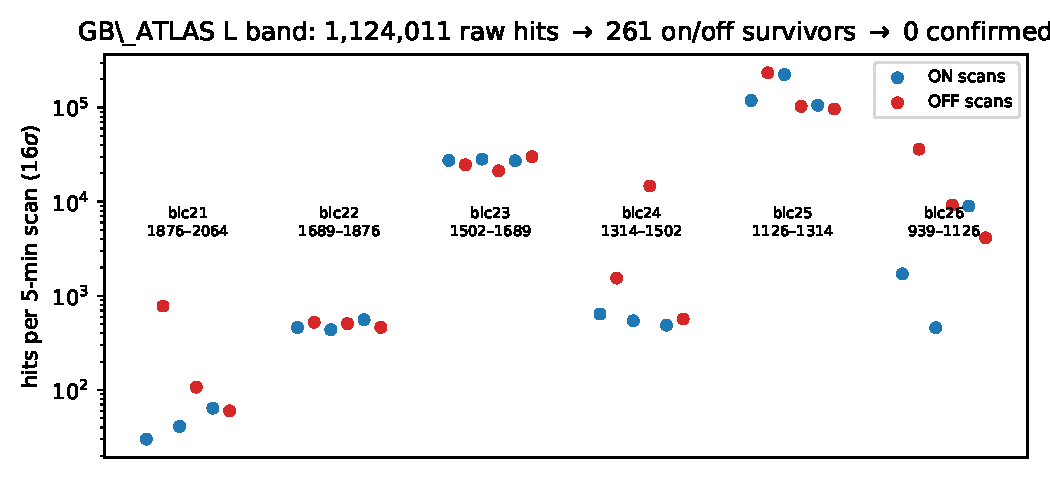
\includegraphics[width=\linewidth]{figures/atlas3i_sweep.pdf}
\caption{Hits per 5-min scan at $16\sigma$ for the six L-band nodes (blue: on-target;
red: off-target), spanning four orders of magnitude with RFI environment. The full
vetting funnel is \aiRawHits\ hits $\to$ \aiSurvivors\ on/off survivors $\to$
\aiConfirmed\ confirmed candidates.}
\label{fig:sweep}
\end{figure}

\software{\code{jansky-research} \citep{janskyresearch}, \code{jansky} \citep{jansky},
NumPy, h5py. Analysis assisted by Claude \citep{anthropicclaude}; all results verified
by the pipeline's test suite.}

\bibliography{refs}
\bibliographystyle{aasjournal}

\end{document}
